\documentclass[a4paper]{article}

\usepackage{INTERSPEECH2021}
\usepackage{subfiles}
\usepackage{datatool}
\usepackage{fmtcount}
\usepackage{xstring}
\usepackage{substr} % Include this in your preamble
\usepackage{tipa}
\DTLloaddb{cronbach}{scripts/data_output/cronbach_alpha.csv}
\DTLloaddb{modelsouts}{scripts/data_output/dynamic_models.csv}
\DTLloaddb{partrem}{scripts/data_output/participant_removal.csv}
\DTLloaddb{taskrem}{scripts/data_output/taskremoval.csv}

\newcommand{\livedata}[2]{%
    \DTLfetch{#1}{Statistic}{#2}{Value}%
}

\title{Measuring music and prosody: accounting for variation in non-native speech discrimination with L1, L2, music skills, and working memory}
%Paper submission must be anonymous. Only fill in author information for the final PDF.
\name{Author Anonymous$^1$, 
Co-author Anonymous$^1$,
Co-author Anonymous$^1$,
Co-author Anonymous$^1$}
%The maximum number of authors in the author list is twenty. If the number of contributing authors is more than twenty, they should be listed in a footnote or in acknowledgement section, as appropriate.
\address{
  $^1$Author Affiliation}
\email{author@university.edu, 
coauthor@company.com}

\begin{document}

\maketitle
% 
\begin{abstract}
The dynamics of non-native speech perception remain poorly understood, especially in accounting for specialized skills/training. One such skill, musical ability, has been shown to positively impact sensitivity to speech sounds, yet how musical ability is operationalized and measured varies from study to study. Individuals’ musical abilities vary in exposure-duration, skill type (e.g., voice, percussion), and skill-level. Here, we take an individual differences (n=38) approach to explore sensitivity in non-native speech discrimination of prosodic contrasts. We measure language background, general cognitive measures, and three measures of musical ability: auditory-motor temporal integration \cite{Kachlicka_Saito_Tierney_2019}, auditory discrimination \cite[MET;]{Wallentin_Nielsen_Friis-Olivarius_Vuust_Vuust_2010}), and musical sophistication \cite[Gold-MSI;]{Müllensiefen_Gingras_Musil_Stewart_2014}. We measured prosodic sensitivity using three AX discrimination tasks and signal detection measures (d'/c): Mandarin tone (primarily cued by pitch), Italian and Japanese (non-)geminates (primarily cued by duration). Results suggest music background, discrimination, and auditory-motor temporal integration capture related –yet divergent– aspects of music experience. Additionally, music sub-skills (e.g., pitch perception) have unequal contributions to non-native speech sensitivity across languages' respective linguistic cues (e.g., tone). Findings support models of non-native speech perception, which consider cognitive factors and auditory experience outside of language experience.

\end{abstract}
\noindent\textbf{Index Terms}:  Individual differences, Music, Non-native speech perception, Measuring prosody

\section{Outline}
\subfile{outline.tex}
\subfile{outline.tex}

\begin{enumerate}
  \item To what extent do various measures of musical experience and skill predict sensitivity to Italian and Japanese geminate contrasts and Mandarin tonal contrasts?
  \begin{itemize}
  \item To what extent do different rhythmic tasks predict Japanese and Italian Geminate Sensitivity?
  \item To what extent do different rhythmic tasks predict Japanese and Italian Geminate Sensitivity?
\end{itemize}
  \item To what extent does language experience deferentially predict sensitivity to Italian and Japanese geminate contrasts and Mandarin tonal contrasts?
  \item To what extent does domain general cognitive abilities deferentially predict sensitivity to Italian and Japanese geminate contrasts and Mandarin tonal contrasts?
\end{enumerate}

\section{methods}

\subsubsection{participants}
 The recruitment of \livedata{partrem}{starting_participants} participants was managed through Prolific \cite{Palan_2018} (n=\livedata{partrem}{data_exp_142778-v2.before})  and in-person (n=\livedata{partrem}{data_exp_141883-v12.before}) recruitment. Additionally, 22 potentional participants were rejected from participation due to failing initial requirements (i.e., eight removed for failed headphone-check \cite{milne_2021} and 14 removed for eye-tracking calibration failure, which is not reported here). To ensure data quality and maximize retained participants, three median absolute deviations (MAD) from median score was calculated as the standard for removal for each task \cite{Leys_2013}. Of the \livedata{partrem}{starting_participants} participants who remained, \livedata{partrem}{removed_participants} were removed for low accuracy scores. Of these, \livedata{taskrem}{particip_remove_lang.remove} were removed for being below MAD range in the language tasks and \livedata{taskrem}{rhythm_part.remove} removed for low performance in auditory-motor integration task.  After removal, \livedata{partrem}{kept_participants} participants (age: $\mu$ = \livedata{partrem}{mean_age}, $\sigma$ = \livedata{partrem}{sd_age}) data were retained for analysis. 

\subsubsection{procedure}
All of the participants took part in a multi-stage battery of language, music, and domain general tasks. Participants first took part in a two-part headphone check, an aural attention check and a dichotic-pitch task \cite{milne_2021}, followed by an 8 trial adaptive staircase digit-span task. After completing the head-phone check and digit-span tasks,
all participants took part in either music or language segments, followed by the complementary segment (i.e., music $\rightarrow$ language, language $\rightarrow$ music). For all language and music tasks, stimuli and experimental design were adapted and built in Gorilla \cite{gorilla_Anwyl-Irvine_2019} for the current study from previous in-person studies (e.g., Mandarin \cite{Wiener_Bradley_2020}) that either made materials openly available on OSF \cite{OSF} or were provided by the original authors. 

In the language segment, participants took part in three speeded AX-discrimination tasks for Italian, Japanese, and Mandarin (trials automatically proceeded after 1000 ms if not responded to)\cite{Hayes‐Harb_Barrios_2021}. All Language stimuli were sampled at 44.1 kHz and recorded in sound attenuated booths (Mandarin) or studio (Japanese and Italian). The Italian and Japanese AX tasks, adapted from \cite{Tsukada_Cox_Hajek_Hirata_2017}, consisted of stop geminate contrasts: Italian - /\textipa{p t k b d g dZ}/, Japanese - /\textipa{t k tS}/. For the Italian AX task, stimuli consisted of 27 pairs of geminate contrasts (e.g., without geminate /\textipa{Eko}/ \textit{echo}, with geminate /\textipa{Ek\textlengthmark o}/ \textit{here}), which were made up of approximately half real and non-real words, spoken by three native speakers. For the Japanese AX task, stimuli consisted of 33 pairs of geminate contrasts, with approximately half of the geminate and non-geminate pairs matching in pitch accent (e.g., without geminate low-high pitch accent /heta/ \textit{unskilled}, without geminate low-high pitch accent /hetːa/ \textit{decreased}) and mismatching in pitch-accent (e.g., without geminate high-low pitch accent /kate/, with geminate low-high pitch accent /katːe/). The Mandarin task, adpated from \cite{Wiener_Bradley_2020}, consisted of 8 stimuli based on the Mandarin syllable yu with four tones (yu1, yu2, yu3, yu4) recorded by male and female native speakers and were normalized for F0 manipulation using \cite{Boersma_Weenink}'s method. Each tonal pairing co-occured equal amounts with each tone occurring with itself three times to equalize match-mismatch answers across the task. 

The music segment has two basic tasks: auditory-motor temporal integration \cite{Kachlicka_Saito_Tierney_2019} and auditory discrimination \cite[MET]{Wallentin_Nielsen_Friis-Olivarius_Vuust_Vuust_2010}, both of which have melody and rhythm sections. In the auditory-motor integration tasks, participants hear a rhythm (auditory-motor rhythm) or melody (auditory-motor rhythm) three times, memorizes it, and reproduces either the melodic or rhythmic phrase. For example, in the auditory-motor rhythm task each trial plays a 13 beat rhythm three times. The participant then needs needs to repeat the exact beat using the space-bar. Timing is captured on each space-bar press. Similarly, for the auditory-motor melody task a series of 7 notes are played, the participants then needs to repeat these with a series of on-screen buttons that correspond to relative pitches (always starts in the middle). After completion of both auditory-motor temproal integration tasks, the participant then does a rhythm and melody Musical Ear task \cite{Wallentin_Nielsen_Friis-Olivarius_Vuust_Vuust_2010} (auditory AX discrimination task), where two auditory music samples (melody or rhythm) are played then participants must determine if the samples were identical (melodies or drum beats) through a button press on the screen. 

After completing the music and language segments, participants then fill in both a musical sophistication survey \cite[Gold-MSI;]{Müllensiefen_Gingras_Musil_Stewart_2014} and a Language Experience and Proficiency Questionnaire (LEAP-Q) \cite{Marian_Blumenfeld_Kaushanskaya_2007}. The Goldsmiths-MSI is a self-reported survey, which aims to capture individual differences through musical sophistication in 5 areas: Active Musical Engagement (e.g., time and money resources spent on music); Self-reported Perceptual Abilities (e.g., musical listening skills); Musical Training (e.g. formal musical training); Self-reported Singing Abilities (e.g. one’s own singing); Emotional Engagement with Music (e.g. ability to talk about emotions in music). Finally, the participant fills out the LEAP-Q with self-reported data on their language proficiency and experience of bilingual and multilingual practices. 

\subsection{Data Analysis}
\subsubsection{Data Wrangling and Validation}


Reaction time based data removal was calculated by overall trial log transformed reaction time on both the musical ear tasks (rhythm and melody). MAD was used as the removal standard, reaction time trial data outside three deviations was removed (proportion of trials removed from musical ear tasks: \livedata{taskrem}{RTmet.remove} of \livedata{taskrem}{RTmet.before} trials). Language tasks were transformed using the squareroot transformation due to larger skew that is likely due to the speeded nature of the AX tasks. No trials data was removed from language tasks due to the automatic progression of trials at 1000ms.

Data removal based on accuracy was then calculated by item for both Musical Ear tasks and for each language task. The standard of three MADs was applied to each task's accuracy. Removal was conservative for each task, retained items for each task: Auditory-motor melody items \livedata{taskrem}{melody_item.after}/\livedata{taskrem}{melody_item.before}, Auditory-motor rhythm items \livedata{taskrem}{rhythm_item.after}/\livedata{taskrem}{rhythm_item.before}, Mandarin items \livedata{taskrem}{Mandarin.after}/\livedata{taskrem}{Mandarin.before}, Italian items \livedata{taskrem}{italian.after}/\livedata{taskrem}{italian.before}, Japanese items \livedata{taskrem}{japanese.after}/\livedata{taskrem}{japanese.before}. Additionally in the auditory-motor rhythm task, the first beat of every trial (rhythmic phrase) was removed. This was done because the first beat acted as the trigger for beginning the capture of rhythm. As each possible beat is 200 ms apart, the second beat of each rhythmic phrase was then centered by subtracting 100 ms, as seen in fig \ref{fig:beat_data}

\begin{figure}[t]
  \centering
  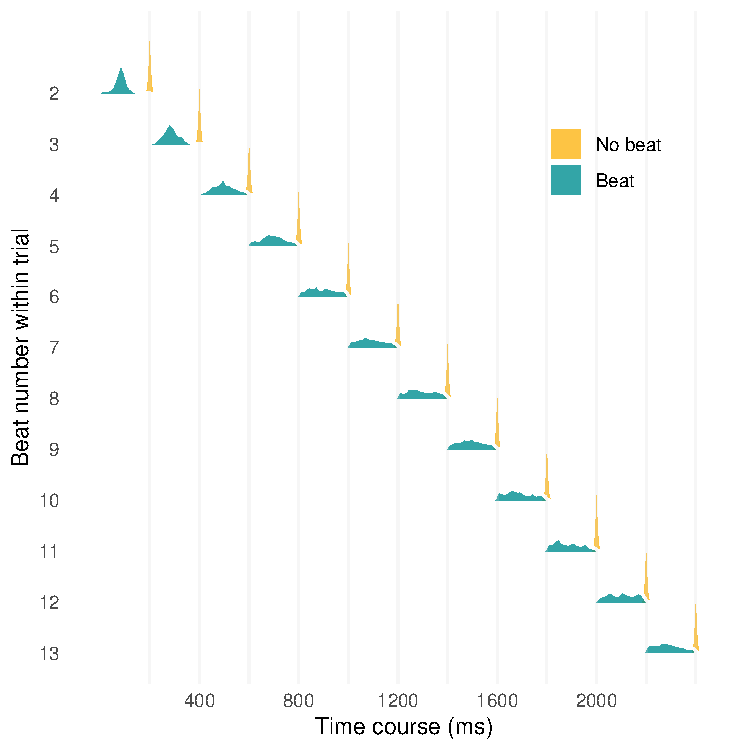
\includegraphics[width=\linewidth]{SP_24_visuals/Correct_and_Incorrect_distrubutions_by_beat_across_trial.pdf}
  \caption{distribution of beats hit (space bar) over trials. Timing frames for each of beat (2-13) is illustrated by horizontal lines. No-beat distributions represent \cite{gorilla_Anwyl-Irvine_2019}'s measurement sensitivity}
  \label{fig:beat_data}
\end{figure}

After data removal, Cronbach's alpha was calculated for each of the musical tasks and questionnaire as tested in original studies (i.e., Goldsmiths 5 area scores, \textit{Musical Ear Task} melody and rhythm items, auditory-motor melody, auditory-motor rhythm) to test internal reliability of items in each task. Results as compared to original studies are presented in Table~\ref{tab:comparison}. 

\begin{table}[ht]
\centering
\begin{tabular}{|c|c|c|}
\hline
\textbf{Task} & \textbf{Reported Value} & \textbf{Our Value} \\
\hline
GoldSmiths \cite{Müllensiefen_Gingras_Musil_Stewart_2014} & Range: 0.79 - 0.93 & 0.89 \\
Musical Ear tasks \cite{Wallentin_Nielsen_Friis-Olivarius_Vuust_Vuust_2010}& 0.87 & 0.79 \\
Auditory-motor melody \cite{Kachlicka_Saito_Tierney_2019}& Unreported & 0.93 \\
Auditory-motor rhythm\cite{Kachlicka_Saito_Tierney_2019}& Unreported & 0.91 \\
\hline
\end{tabular}
\caption{Comparison of reported Cronbach's alpha values compared to our Cronbach's alpha values}
\label{tab:comparison}
\end{table}

For both Musical Ear tasks and each Language task,  D-prime (d′) was calculated as a measure of sensitivity and to account for AX-discrimination response bias \cite{Macmillan_Creelman_2004}. Figure \ref{fig:dprime} shows Language D-prime by matching L2 (i.e., has studied the respective language) and basic music experience (i.e. does or does not actively play an instrument/sing). 

\begin{figure}[t]
  \centering
  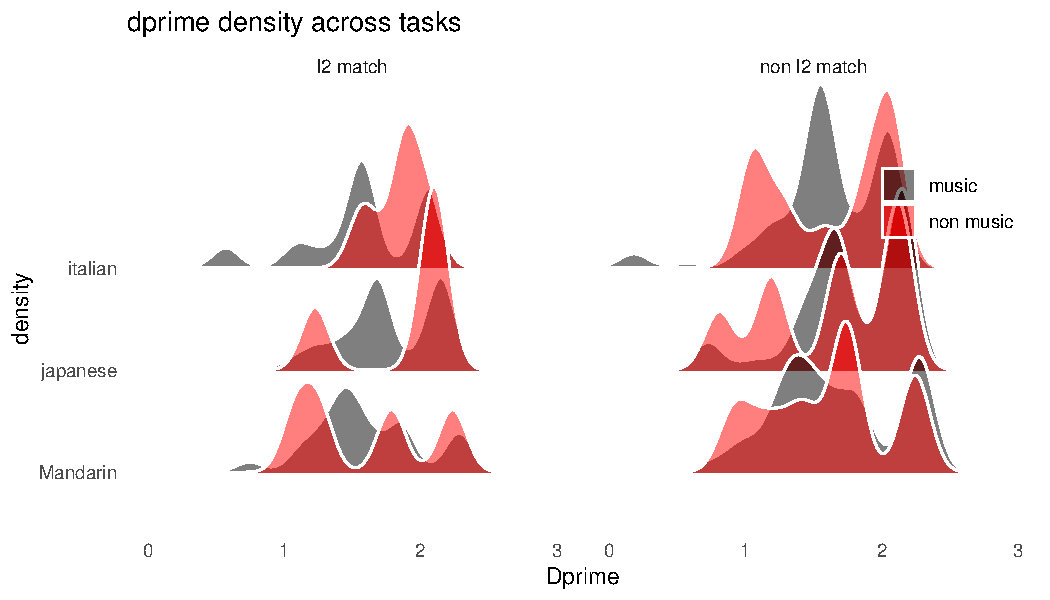
\includegraphics[width=\linewidth]{SP_24_visuals/dprime_density_across_tasks.pdf}
  \caption{Raw data}
  \label{fig:dprime}
\end{figure}

\subsubsection{statistical analysis}


All quantitative variables from each of the tasks were centered on their mean to 0 and normalized so that the scale of individual variables was similar across tasks (Goldsmiths general, Goldsmiths engagement, Goldsmiths perception, Goldsmiths training, Goldsmiths singing, Goldsmiths emotions, Musical Ear Test d' Melody, Musical Ear Test d' Rhythm","Working-memory, Auditory-motor Rhythm, Auditory-motor Melody), as seen in figure \ref{fig:centered_data}.

\begin{figure*}[t]
  \centering
  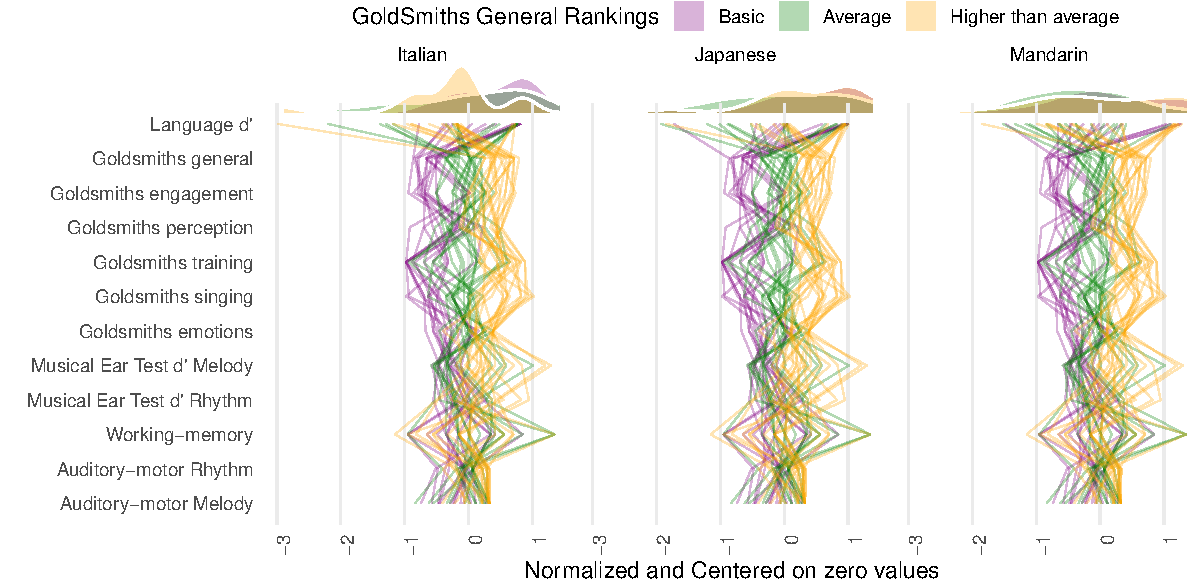
\includegraphics[width=\textwidth]{SP_24_visuals/by_gs.pdf}
  \caption{Raw data}
  \label{fig:centered_data}
\end{figure*}

To test how various measures of musical experience and skill, language experience, and domain general cognitive abilities differentially affect Italian and Japanese geminate contrast sensitivity and Mandarin tone sensitivity, three multiple linear regression models were built to compare the relative contribution of each task on centered D-prime scores of each language. Maximal Models were built using the \textit{lm} package \cite{lmPackage} in R \cite{RManual}. Each model included 14 predictor effects: L1 (coded as match no match), L2 (coded as match no match), Music student (coded as does or does not actively play an instrument/sing), Goldsmiths general, Goldsmiths engagement, Goldsmiths perception, Goldsmiths training, Goldsmiths singing, Goldsmiths emotions, Musical Ear Test d' Melody, Musical Ear Test d' Rhythm, Working-memory, Auditory-motor Rhythm, Auditory-motor Melody). All variables were coded with effects coding. Models were reduced in the following order: removal of non theoretical driven music skill (e.g., rhythm for Mandarin and Melody for Italian and Japanese), then effects were removed based on how much variance was explained in terms of coefficients and post hoc colinearity. Japanese and Mandarin models, were reduced minimally due to finding early evidence of parsimonious models. For the Italian models, no model came out significantly better. the Model was reduced until all co-linearity was no longer apparent in model comparison. 

An effect of Musical Ear Task rhythm or auditory-motor rhythm would indicate that rhythmic ability predicts sensitivity in a language, whereas an effect of Musical Ear Task melody or auditor-motor melody would indicate that melody ability predicts sensitivity in a language. Further, an effect of Musical Ear Task would suggest that perceptive means of measuring music have a larger predictive power, whereas an effect found from auditory-motor tasks would suggest that productive musical measures hold more predictive power. Results from the Mandarin Linear model found significant effects for: GoldSmiths emotions ($\beta$ = \livedata{modelsouts}{Mandarin.gs_emotions.estimate}, \text{SE} = \livedata{modelsouts}{Mandarin.gs_emotions.std.error}, z = \livedata{modelsouts}{Mandarin.gs_emotions.statistic}, p < \livedata{modelsouts}{Mandarin.gs_emotions.p.value}), indicating that higher musical emotional ratings for predict lower sensitivity to Mandarin tone; Musical Ear Test melody ($\beta$ = \livedata{modelsouts}{Mandarin.MET_dprime_melody.estimate}, \text{SE} = \livedata{modelsouts}{Mandarin.MET_dprime_melody.std.error}, z = \livedata{modelsouts}{Mandarin.MET_dprime_melody.statistic}, p $<$ \livedata{modelsouts}{Mandarin.MET_dprime_melody.p.value}), indicating that higher perceptual sensitivity to musical pitch predicts higher sensitivity to Mandarin tone. 

Results from the Italian Linear model found significant effects for: GoldSmiths general ($\beta$ = \livedata{modelsouts}{Italian.gs_general.estimate}, \text{SE} = \livedata{modelsouts}{Italian.gs_general.std.error}, z = \livedata{modelsouts}{Italian.gs_general.statistic}, p < \livedata{modelsouts}{Italian.gs_general.p.value}), indicating that higher musical emotional ratings for predict lower sensitivity to Mandarin tone; Musical Ear Test melody ($\beta$ = \livedata{modelsouts}{Italian.MET_dprime_melody.estimate}, \text{SE} = \livedata{modelsouts}{Italian.MET_dprime_melody.std.error}, z = \livedata{modelsouts}{Italian.MET_dprime_melody.statistic}, p $<$ \livedata{modelsouts}{Italian.MET_dprime_melody.p.value}), indicating that higher perceptual sensitivity to musical pitch predicts higher sensitivity to Mandarin tone.

all of our fancy results

~\ref{fig:model}.

\begin{figure}[t]
  \centering
  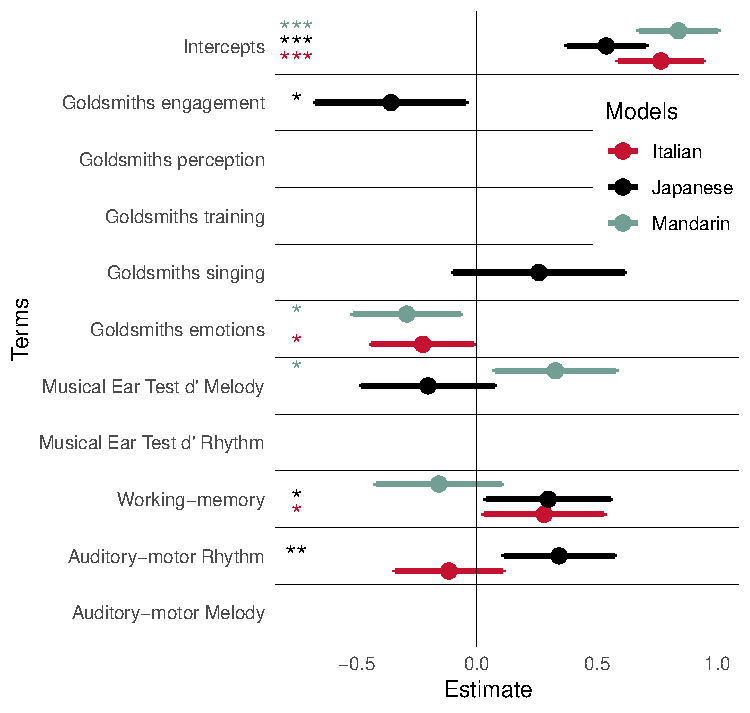
\includegraphics[width=\linewidth]{SP_24_visuals/Japanese,Italian,_Mandarin_max_models_structure:_parsimonious_effects.pdf}
  \caption{model output}
  \label{fig:model}
\end{figure}

\section{Discussion}

\section{Conclusions}

Complex measurement stuff. But, still many things to discover

\section{Acknowledgements}

We would like to thank XXXX and XXXX for funding this project. Additionally, we would like to thank the language instructors that allowed us to recruit in their classrooms\\

\bibliographystyle{IEEEtran}

\bibliography{my_references.bib}

\end{document}
